\documentclass[12pt, letterpaper]{elsarticle}
\usepackage[utf8]{inputenc}
\usepackage{graphicx}

\title{Neutronics aspects of the FESS-FNSF}
\author[wisc]{A. Davis\corref{cor1}}
\ead{andrew.davis@wisc.edu}
\author[wisc]{M. Harb}
\ead{mharb@wisc.edu}
\author[wisc]{L. El-Guebaly}
\ead{elguebaly@wisc.edu}
\author[wisc]{P. Wilson}
\ead{paul.wilson@wisc.edu}
\author[wisc]{E. Marriott}
\ead{marriott@wisc.edu}
\ead[url]{http://cnerg.wisc.edu}
\cortext[cor1]{Corresponding author}

\address[wisc]{1500 Engineering Drive, Madison, WI 53706}
 
\begin{document}
 
\begin{abstract}
Neutronics analysis was performed on the latest Fusion Energy System Studies - Fusion Neutron Science Facility (FESS-FNSF) design which covered the neutron wall loading, tritium breeding ratio, radiation damage, and shutdown dose rate calculations. Sixteen different sector configurations were investigated with a main focus on determining the impact which each has upon the Tritium Breeding Ratio (TBR) of the whole facility.

\vspace{5mm}
\noindent
Keywords: FESS-FNSF, TBR, radiation damage, SDDR
\end{abstract}

\begin{titlepage}
\maketitle
\end{titlepage}

\newpage
\listoffigures

\newpage
\section{Introduction}
The Fusion Energy Systems Studies Fusion Nuclear Science Facility (FESS-FNSF \cite{ref_1}) is considered an essential element of the US fusion roadmap that displays a strategic  pathway from ITER, to US DEMO, and eventually to the first commercial power plant. A FNSF will help bridge the research gap between ITER - low radiation damage, short pulses, no tritium breeding - and DEMO which is designed to operate at power plant relevant fusion parameters. The FNSF will advance the understanding of fusion nuclear sciences (FNS) by providing an integrated platform for establishing a database on all components up to relevant parameters (e.g. 40-60 dpa, blanket temperatures 500-600 C) via in-depth investigation of issues related to Plasma boundary interface (materials interaction with high energy neutron flux, surface/volumetric heating, radiation damage, and gas production), operating in power plant relevant fusion core conditions (temperatures, coolant/breeder flow rates, pressures/stresses, B-field, and neutrons), tritium breeding/extraction/processing, advancing and demonstrating plasma technologies that support very long duration operations, etc.  

This paper describes the stages of nuclear analysis that serve to prove the radiation derived attributes of the system.

\subsection{Configuration}
The systems studies calculations performed have lead to a radial build which defines the material basis for these calculations.
\subsection{Full 3D Build}
The radial build calculation defines the major materials and dimensions that produce the 3D assembly CAD model shown in Figure \ref{fig:cad_fess_fnsf_3d}.
\begin{figure}[h!]
  \centering
  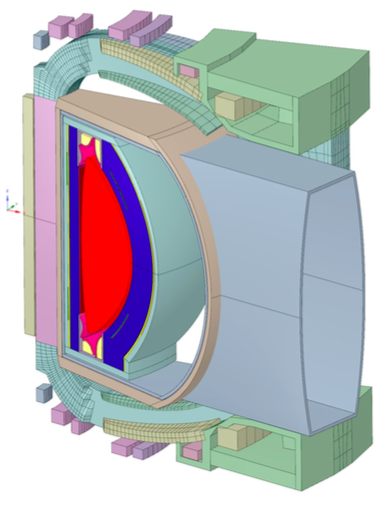
\includegraphics[scale=0.4]{../plots/fess_fnsf_3d_cad.png}
  \caption{The full 3D CAD model of a single FESS-FNSF sector}
  \label{fig:cad_fess_fnsf_3d}
\end{figure}

\section{Analysis Tools}
DAG-MCNP5 coupling
\subsection{Neutron Source Modelling}
Analytic source

\section{Neutron Wall Loading}
Calculations FWs and Divs

\section{Tritium Breeding Calculations}
Introduction
importance of accurate measurements of TBR
\subsection{TBR Workflow}
workflow steps
\subsection{Penetrations and Ports}
figure and results
\subsection{Li-6 Enrichment}
One of the advantages of the DCLL blanket is allowing the control of the T bred by controlling the  Li6 enrichment in LiPb in the main flow channels. Controlling Li6 enrichment is necessary to avoid dealing with a surplus or shortage of T. Analyses were performed to test the effect of changing Li6 enrichment on the overall TBR of the facility (with all penetrations and ports included) and it was found that the TBR dropped to 1.0191 +/- 0.03%, 0.9892 +/- 0.03%, and 0.9513 +/- 0.03% for 70%, 60%, and 50% Li6  enrichment, respectively. The TBR satisfies the tritium breeding requirement of 1.04 with ~ 80% Li6 enrichment and the results are shown in figure 6.
\begin{figure}[h!]
  \centering
  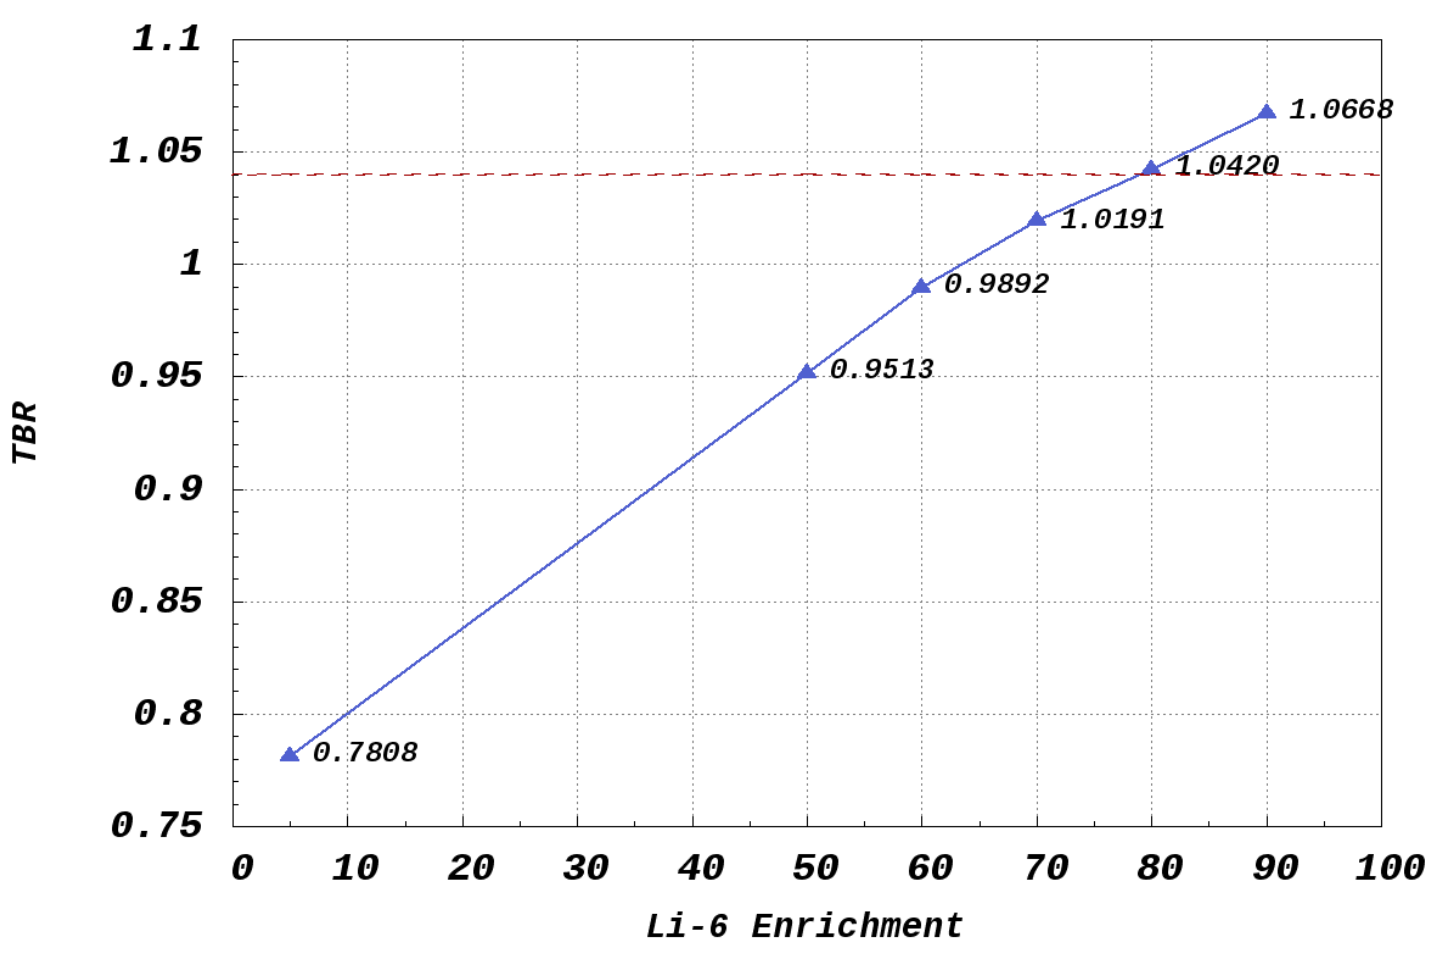
\includegraphics[scale=0.25]{../plots/Li6_enrichment.png}
  \caption{The facility overall TBR vs Li6 enrichment}
  \label{fig:Li6_enrichment}
\end{figure}
chart
\subsection{TBR mapping}
mapping of NBI, step 7, LH
importance of middle region
\section{Radiation Damage}
\subsection{dpa, He/H production}
at FW and radial distribution of damage
\subsection{Magnet damage}
fast neutron fluence, heating, dpa to Cu stabilizer

\section{Shutdown Dose Rate Calculations}
introduction and r2s worflow
\subsection{SDR}
\subsection{Decay Heat}

\newpage
\section{References}
\begin{thebibliography}{10} 
\bibitem{ref_1} 
C. E. KESSEL, et al, {“The Fusion Nuclear Science Facility, the Critical Step in the Pathway to Fusion Energy,” Fusion Science and Technology, vol. 68, p. 225–236 (2015).}
\end{thebibliography}

\end{document}